\documentclass{beamer}

\usetheme[secheader]{Boadilla}
\usecolortheme{beetle}
\usepackage[latin1]{inputenc}
\usepackage{listings} % for code syntax highlighting
\usepackage{color}

\usepackage{inconsolata} % for code
\usepackage{lmodern}
\renewcommand*\familydefault{\sfdefault} 
%\usepackage[T1]{fontenc}
%\usepackage[default]{gfsneohellenic}
 
\definecolor{dkgreen}{rgb}{0,0.6,0}
\definecolor{gray}{HTML}{3A3A3A}
\definecolor{mauve}{rgb}{0.58,0,0.82}
\definecolor{codebg}{HTML}{1C1C1C}
\definecolor{codefg}{HTML}{D0D0D0}
\definecolor{codekeyword}{HTML}{87AFDF}
\definecolor{codecomment}{HTML}{808080}
\definecolor{pastelred}{HTML}{DF8787}

\definecolor{javared}{rgb}{0.6,0,0} % for strings

% tweak beamer theme
%\setbeamercolor{background canvas}{bg=gray}
 
% tweak listings for code ==================
\lstset{ %
  language=C++,                % the language of the code
  basicstyle=\small\ttfamily\color{codefg},           % the size of the fonts that are used for the code
  %numbers=left,                   % where to put the line-numbers
  %numberstyle=\tiny\color{gray},  % the style that is used for the line-numbers
  %stepnumber=2,                   % the step between two line-numbers. If it's 1, each line 
                                  %% will be numbered
  %numbersep=5pt,                  % how far the line-numbers are from the code
  backgroundcolor=\color{codebg},      % choose the background color. You must add \usepackage{color}
  showspaces=false,               % show spaces adding particular underscores
  showstringspaces=false,         % underline spaces within strings
  showtabs=false,                 % show tabs within strings adding particular underscores
  %frame=single,                   % adds a frame around the code
  rulecolor=\color{black},        % if not set, the frame-color may be changed on line-breaks within not-black text (e.g. commens (green here))
  tabsize=2,                      % sets default tabsize to 2 spaces
  captionpos=b,                   % sets the caption-position to bottom
  breaklines=true,                % sets automatic line breaking
  breakatwhitespace=false,        % sets if automatic breaks should only happen at whitespace
  title=\lstname,                   % show the filename of files included with \lstinputlisting;
                                  % also try caption instead of title
  keywordstyle=\color{codekeyword}\bfseries,
  stringstyle=\color{javared},
  commentstyle=\color{codecomment},
  escapeinside={\%*}{*)},            % if you want to add LaTeX within your code
  morekeywords={*,...}               % if you want to add more keywords to the set
}
% ==========================================

\title{Forgetting the C in C++}
\author{Alexander Kondratskiy}
\date{\today}
% \institute[2008]{ECON 101}

\begin{document}

\frame{\titlepage}

\section{Introduction}
\frame{\sectionpage}

\frame {
    \frametitle{What is the talk about?}
    \begin{itemize}
        \item<2->Overview of C++, from a C programmer's perspective
        \item<2->Good C++ coding style
        \item<2->More than "C with classes"
        \item<2->Fixing bad habbits learnt from C.
    \end{itemize}
}

\frame {
    \frametitle{Motivation}
    \begin{itemize}
        \item<1->C++ has evolved
            % TODO: find word 
        \item<2->\alert{Safety}/
            \begin{itemize}
                \item Resource management (including memory)
                \item Type safety
                \item Compiler checks
            \end{itemize}
        \item<2->\alert{Readability}/maintainability
            \begin{exampleblock}{}
                ``Programs must be written for people to read, and only incidentally for machines to execute.''
                \hspace*\fill{\small--- Abelson/Sussman, SICP}
            \end{exampleblock}
        \item<2->Programmer \alert{Productivity}
            \begin{itemize}
                \item STL
                \item Abstractions
            \end{itemize}
        \item<2->\alert{Efficiency} and speed
            \begin{itemize}
                \item More context for compiler
            \end{itemize}
        \item<3->Win-win
    \end{itemize}
}

\frame {
    \frametitle{Method}
    \begin{itemize}
        \item<1->Observe common C idiom
        \item<1->Discuss disadvantages
        \item<1->C++ alternative
        \item<1->Gains from the alternative
        \item<2->Learn new techniques/features along the way
    \end{itemize}
}

\section{Prerequisites}
\frame{\sectionpage}

\begin{frame}
    \frametitle{History of C++}

    %\renewcommand\windowpagestuff{%
        %\hfill
        %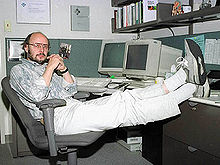
\includegraphics[height=3cm]{220px-BjarneStroustrup.jpg}
        %%\par{\usebeamercolor[fg]{caption name}%
            %%\usebeamerfont*{caption name}\figurename%
        %%\usebeamertemplate{caption label separator}}%
        %%\raggedright%
        %%\usebeamerfont*{caption}%
        %%Bjarne Stroustrup%
    %}

    %\opencutright

    \begin{columns}[t]
        \column{7cm}
        \begin{itemize}
            \item<1->Started by Bjarne Stroustrup in 1979 as "C with Classes"
                \begin{itemize}
                    \item At Bell labs
                    \item "Down the hall" from Dennis Ritchie (creator of C)
                \end{itemize}
            \item<1->Renamed to C++ in 1983, commercially implemented in 1985
            \item<2->1990s: stream IO, STL, ISO Standard in 98
            \item<3->2000s: Boost, TR1 in 2007
            \item<4->2010s: C++11 in 2011
        \end{itemize}
        \column[T]{4cm}
        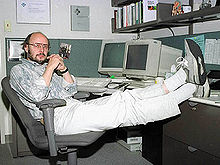
\includegraphics[width=4cm]{220px-BjarneStroustrup.jpg}
    %\end{columns}
    %\begin{columns}[t]
        %\column{11cm}
    \end{columns}

    %\begin{cutout}{0}{.65\linewidth}{0pt}{6}
    %\end{cutout}
\end{frame}

\begin{frame}
    \frametitle{C Compilation model}
    \framesubtitle{A single source file}
    \begin{columns}[t]
        \column{4cm}
        \begin{itemize}
            \item One source file at a time
            \item Preprocessor \emph{resolves all directives}
            \item Compiled to an object file
            \item Missing external function definitions
        \end{itemize}
        \column[T]{8cm}
        \includegraphics[width=7cm]{diagrams/c_compilation_model.png}
    \end{columns}
\end{frame}

\begin{frame}
    \frametitle{C Compilation model}
    \framesubtitle{Linking}
    \begin{columns}[t]
        \column{4cm}
        \begin{itemize}
            \item Linker combines several translation units
            \item Resolves external dependencies
        \end{itemize}
        \column[T]{8cm}
        \includegraphics[height=9cm,angle=-90]{diagrams/c_compilation_model_linker.pdf}
    \end{columns}
\end{frame}

\begin{frame}
    \frametitle{C Compilation model}
    \framesubtitle{A typical project}
    \includegraphics[height=12cm,angle=-90]{diagrams/c_compilation_model_full.pdf}
\end{frame}

\begin{frame}
    \frametitle{\alert{C++} Compilation model}
    \begin{itemize}
        \item Same as C compilation model
        \item Template instantiation happens in the compiler
    \end{itemize}
\end{frame}

% define a counter for rules
\newcounter{rulecount}
\newcommand{\declarerule}{
    \textbf{\alert{Rule \therulecount:}}
}

\section{Preprocessor}
\frame{\sectionpage}

\begin{frame}
    \frametitle{\declarerule Avoid the preprocessor}
    \begin{itemize}
        \item Macros are text substitution
        \item Macros not subject to scope rules
        \item Compiler does not see any preprocessor directives only final result of substitution
            \begin{itemize}
                \item No meaningful error checking!
            \end{itemize}
        \item Used naively can lead to subtle, hard to find bugs
    \end{itemize}
\end{frame}

\stepcounter{rulecount}
\begin{frame}[fragile]
    \frametitle{\declarerule Avoid \#define constants}
\begin{lstlisting}
#define DAYSINWEEK 7
for (i = 0; i < l; ++i) {
    printf("i: %d\n", i);
}
\end{lstlisting}
    \begin{itemize}
        \item Macros are text substitution
        \item Compiler does not see any preprocessor directives
        \itemize{
            \item No meaningful error checking!
            }
    \end{itemize}
\end{frame}

\stepcounter{rulecount}
\begin{frame}[fragile]
    \frametitle{\declarerule Avoid macro functions}
Given an innocent macro definition:
\begin{lstlisting}
#define CIRCLE_AREA(RADIUS) 3.14 * RADIUS * RADIUS
\end{lstlisting}
You write:
\begin{lstlisting}
double area = CIRCLE_AREA( a + b );
\end{lstlisting}
The compiler sees:
\begin{lstlisting}
double area = 3.14 * a + b * a + b;
\end{lstlisting}
\end{frame}

% Fixing macro problem with brackets
\begin{frame}[fragile]
    \frametitle{\declarerule Avoid macro functions}
    \textbf{Macro Solution:} Wrap arguments in brackets:
\begin{lstlisting}
#define CIRCLE_AREA(RADIUS) 3.14 * (RADIUS) * (RADIUS)
\end{lstlisting}
\begin{itemize}
    \item This is just a bandaid
\end{itemize}
    \textbf{Better solution:} inline functions:
\begin{lstlisting}
inline double circle_area(double radius) {
    return 3.14 * radius * radius;
}
\end{lstlisting}
\begin{itemize}
    \item Type safe
    \item Checked by compiler
    \item Scope
\end{itemize}
\end{frame}

% Demonstrate problem with multiline macros
\begin{frame}[fragile]
    \frametitle{\declarerule Avoid macro functions}
\begin{lstlisting}
#define CIRCLE_AREA(RADIUS) 3.14 * (RADIUS) * (RADIUS)
\end{lstlisting}
\end{frame}

\end{document}
